\documentclass{article}
\usepackage[utf8]{inputenc}
\usepackage[margin=0.5in,includefoot]{geometry}
\usepackage[export]{adjustbox}

% Header and Footer Setup
\usepackage{fancyhdr}
\pagestyle{fancy}
\fancyhead{}
\fancyfoot{}
\fancyfoot[R]{\thepage}
\renewcommand{\headrulewidth}{0pt}
\renewcommand{\footrulewidth}{0pt}
%
%Graphics Setup
\usepackage{graphicx}
\usepackage{float}
\usepackage{subfig}


%list setup
\usepackage{amssymb}
\renewcommand{\labelitemi}{$\blacktriangleright$}
\renewcommand{\labelitemii}{$\bullet$}
\renewcommand{\labelitemiii}{$\circ$}

%Source Code setup
\usepackage{xcolor}
\usepackage{listings}

\definecolor{mGreen}{rgb}{0,0.6,0}
\definecolor{mGray}{rgb}{0.5,0.5,0.5}
\definecolor{mPurple}{rgb}{0.58,0,0.82}
\definecolor{backgroundColour}{rgb}{0.95,0.95,0.92}

\lstdefinestyle{CStyle}{
    backgroundcolor=\color{backgroundColour},   
    commentstyle=\color{mGreen},
    keywordstyle=\color{magenta},
    numberstyle=\tiny\color{mGray},
    stringstyle=\color{mPurple},
    basicstyle=\footnotesize,
    breakatwhitespace=false,         
    breaklines=true,                 
    captionpos=b,                    
    keepspaces=true,                 
    numbers=left,                    
    numbersep=5pt,                  
    showspaces=false,                
    showstringspaces=false,
    showtabs=false,                  
    tabsize=2,
    language=C
}
%


\begin{document}

\begin{titlepage}

	\begin{flushright}
	\textsc{\large April 22, 2021} \\
	\end{flushright}
	\begin{center}
	\Large{\bfseries GTU Department of Computer Engineering \\ CSE344 - Spring 2021 \\ Homework 3 Report  } \\
	\end{center}
	\topskip0pt
	\vspace*{\fill}
	\begin{center}
	\Large{\bfseries Akif Kartal \\ 171044098 }
	\end{center}
	\vspace*{\fill}

\end{titlepage}

\cleardoublepage
\section{Problem Definition}
The problem is to make \textbf{peer-to-peer} communication between N process by using fifo, shared memory and named semaphore. 

\section{Solution}
The homework was finished as expected in homework pdf file. 
\subsection{Some Problems and Solutions}
\subsubsection{Shared Memory Usage}
In order to use shared memory correct way between process I made following struct to keep in shared memory for each process.
\begin{lstlisting}[style=CStyle]
typedef struct potato
{
    pid_t pot_pid;
    int switches;
    char fifo_name[50];
    char real_name[30];
    int done;
    int is_opened;
}player;
\end{lstlisting}
In this struct \textbf{fifo\_name} denotes path of the fifo, \textbf{real\_name} denotes fifo real name such as aliVeliFifo \textbf{done} denotes number of 
switch already made.\\ \\
\textbf{Usage:}
\begin{lstlisting}[style=CStyle]
 data = (player *)mmap(NULL, len, PROT_READ | PROT_WRITE, MAP_SHARED, fd, 0);
 int numberOfSwitch = atoi(givenParams.bArg);
 player info;
 strcpy(info.fifo_name, name);
 strcpy(info.real_name, realt_name);
 info.switches = numberOfSwitch;
 info.pot_pid = getpid();
 info.done = 1;
 info.is_opened = 0;
 memcpy(&data[k - 1], &info, sizeof(info)); 
\end{lstlisting}
\subsubsection{Opening Fifo Deadlock}
In this problem if you try to open a fifo on one side, until other side is open it will waiting on open and no other process can continue, 
if you have not a precaution about that.
\subsubsection{Solution}
In order to solve this problem I used \textbf{posix barrier semaphores} because actually here we have barrier problem. \\ \\
The semaphores that I used;
\cleardoublepage
\begin{lstlisting}[style=CStyle]
    int n = getNumberOfLine(fifoNames);

    /*open given semaphore*/
    sem_t *sem_id = sem_open(givenParams.mArg, O_CREAT, 0666, 1);
    if (sem_id == SEM_FAILED)
        errExit("sem_open error!");

    /*define other semaphores to make synchronization between process*/
    sem_t *sem_count = sem_open("counter", O_CREAT, 0666, n + 1);
    if (sem_count == SEM_FAILED)
        errExit("sem_open error!");
    sem_t *sem_barrier = sem_open("barrier", O_CREAT, 0666, 0);
    if (sem_barrier == SEM_FAILED)
        errExit("sem_open error!");
    sem_t *sem_fifo_barrier = sem_open("fifo_barrier", O_CREAT, 0666, 0);
    if (sem_fifo_barrier == SEM_FAILED)
        errExit("sem_open error!");
\end{lstlisting}
Step by Step solution;
\begin{itemize}
	\item Take the fifo creation, saving into shared memory and opening fifo in critical region by using given semaphore name in arguments.
	\item To solve barrier problem with posix semaphores we need a counter variable which is shared between processes, but the problem here is processes have
	different address space, and I didn't want to use a shared memory for this, therefore I created counter by using an extra named semaphore and initialize it 
	with N+1.
	\item After entering critical region decrement counter semaphore using sem\_wait().
	\item After that, make shared memory and finding unique fifo name operations.
	\item After finding a unique name create the fifo with this name.
	\item After this, by using counter variable if the process is not first process check by using shared memory is there a waiting fifo to open
 	and open it in write mode.
 	\item Then, put a sem\_wait statement for fifo\_barrier semaphore after opening the fifos and wait there until last fifo is created not opened.
 	\item Before, try to open fifo first check by using counter semaphore is this last process, if it is then make a sem\_post for fifo\_barrier semaphore,
 	so that opened processes can continue.
 	\item Also, before, try to open fifo first make a sem\_post for the given critical region semaphore so that other processes can enter critical region.
 	\item And now, try to open fifo for both reading and writing. Note that writing end is opened in order to ensure that the process doesn’t see EOF if all other
 	processes close the write end of the FIFO.
 	\item If the open was succesful and if you pass fifo\_barrier semaphore, lastly check is there any waiting process 
    to open it's fifo, if any open it.
 	\item Then, by checking counter variable if this is the last process, make a  sem\_post for the barrier semaphore and wait for barrier semaphore.
 	\item After passing barrier semaphore, first post a barrier for other process and check the process has a potato or not.
 	\item If it has a potato first send it to another process and wait others.
 	\item If it has not a potato wait others.
\end{itemize}
\textbf{Why I used a barrier semaphore?} \\ \\
In order to sending and receiving messages between processes and fifos everything must be ready. Therefore we need to wait all processes to finish 
their opening and initializing before start to sending and receiving, that's why we have a barrier and counter semaphore before start.
\subsubsection{Critical Regions}
Updating shared memory is an important issue therefore, I took that part into critical region in code by using given semaphore.
\subsubsection{Checking Last Potato}
To check if receiving potato is last one I used shared memory and if it is then I send a message all other processes making message pid -1,
so that if the pid is -1 they will finish their jobs.
\subsubsection{Removing Resources and Exiting}
In order to run a cleaner method after finish, I used \textbf{atexit()} function with a cleaner method like this;
\begin{lstlisting}[style=CStyle]
 /*global names to remove*/
 static char myFifoName[50];
 static char memoryName[50];
 static char semphoreName[50];

 /*remove function before exit*/
 static void removeAll(void)
 {
     unlink(myFifoName);
     sem_unlink(semphoreName);
     sem_unlink("counter");
     sem_unlink("barrier");
     sem_unlink("fifo_barrier");
     shm_unlink(memoryName);
 }
 /*save remove method*/
 if (atexit(removeAll) != 0)
    errExit("atexit");
\end{lstlisting}

\subsubsection{CTRL-C Handling}
In order to give a message on CTRL-C interrupt, I used \textbf{sigaction} function from \textbf{signal.h} library.
Also, I used a \textbf{global variable} to set if an interrupt has occur.
\begin{lstlisting}[style=CStyle]
volatile __sig_atomic_t exitSignal = 0;
void exitHandler(int signal)
{
    if (signal == SIGINT)
    {
        exitSignal = 1;
    }
}
\end{lstlisting}
In each loop in code, signal flag was checked, on interrupt signal, resources was given back and exited elegantly.
\section{System Requirements}
In order to run program you need an ascii file with N rows. Each row must contain a unique fifo name(path).
\textbf{Note that} number of row in file and number of processes must be same. Also, file must contain an empty row at the end of it.
\section{References that was used} 
While doing this howemork following references was used;
\begin{itemize}
	\item Course Textbook Listing 44-7: An iterative server using FIFOs
	\item Week-8 slides synchronization barrier problem with POSIX semaphores.
\end{itemize}
\section{Test Result}
\textbf{Note:} I understand that from pdf it doesn't have to be at least 1 process with zero potatoes. I think there is no such a condition because even though all of them has potato they are sending each other immediately. \\ \\
A simple test result is following;
\begin{figure}[H]
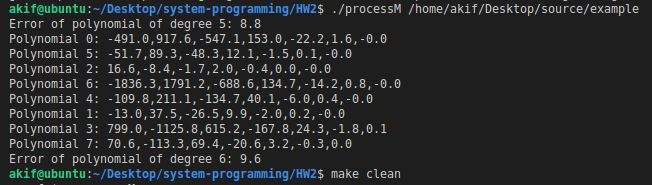
\includegraphics[width=1\textwidth, left]{result.JPG}
\caption[Optional caption]{}
\label{}
		
\end{figure}                              

\end{document}